\section{Paradise Lost}

\begin{quotex}
In the right order of nature, the flesh is subject to the spirit and not the reverse.
\flright{\textsc{The Cloud of Unknowing}}
\end{quotex}


In \emph{Letter III: The Empress} of \textbf{The Meditations on the Tarot}, we learn the three effects of the Fall of Adam:

\begin{itemize}


\item toil

\item suffering

\item death
\end{itemize}


Each of these effects is related to one of the first three Arcana. Chart \ref{tab:EffectsFall} shows what was lost with each effect of the Fall. The ``Good News'' is that each of the effects can be overcome, and the original state restored.

\begin{table}[h]\small\centering
\begin{tabular}{ccc}\toprule
\textbf{Arcanum} & \textbf{Before the Fall} & \textbf{After the Fall} \\\midrule
Magician & Mystical Union with God & Toil \\
High Priestess & Gnosis & Suffering \\
Empress & Sacred magic & Death \\\bottomrule
\end{tabular}
\label{tab:EffectsFall}
\caption{Effects of the Fall}
\end{table}

\begin{itemize}


\item Instead of toil, there was mystical spontaneity.

\item Learning through suffering replaced direct revelation and gnosis.

\item Death entered the domain of life and sacred, creative magic.
\end{itemize}

With these clues, we can return to the first Arcanum of the Magician to unpack it. First of all, the principle of this Arcanum underlies all the others, viz.,

\begin{quotex}
The connection between personal effort and spiritual reality
\end{quotex}


More specifically, the Magician reveals the practical method for this relationship to the other Arcana. It is insufficient to know cognitively; personal effort is also required. The fundamental principle of esoterism, which shows the way to the experience of the reality of the spirit:

\begin{itemize}


\item Learn at first concentration without effort

\item transform work into play

\item make every yoke that you have accepted easy and every burden that you carry light
\end{itemize}


Hence the first practical task is to learn concentration, which is ``the suppression of the fluctuations of the mental substance'' (Patanjali). In practical terms, these fluctuations are the intellectual and sensual imagery that occupies our minds. They arise spontaneously, scattering attention; that is the opposite of concentration.

Calm and silence are the conditions for concentration, when the mind is free of the spontaneously arising images. Therefore, the cultivation of inner silence\footnote{\url{https://gornahoor.net/?p=1082}} is the necessary prelude to any meditation on the Tarot.

If the Magician --- the first Arcanum --- underlies all the other Arcana, then the World --- the last Arcanum --- unifies all the other Arcanum into a Whole. However, it is not so simple, since the World, when analyzed, actually comprises four Worlds. These four worlds are the background for psychurgical practice, leading from the Fallen state back to the State before the Fall. These worlds can be characterized like this:

\begin{itemize}


\item \textbf{Action}: The world of sensual and intellectual imagery.


\item \textbf{Formation}: The destruction of this imagery, i.e., the emptying of the mind.

\item \textbf{Creation}: The Silence necessary to receive Revelation from above.

\item \textbf{Emanation}: Pure creative activity.

\end{itemize}


Do you see how this ties in with the esoteric principle of the Magician?

In the fallen state, the mind is perturbed with the spontaneously arising fluctuations of sensual and intellectual imagery. In this state, the mind is attached to the lowest plane of toil, suffering, and death, as it cannot conceive of anything superior.

\begin{wrapfigure}{rt}{.3\textwidth}
	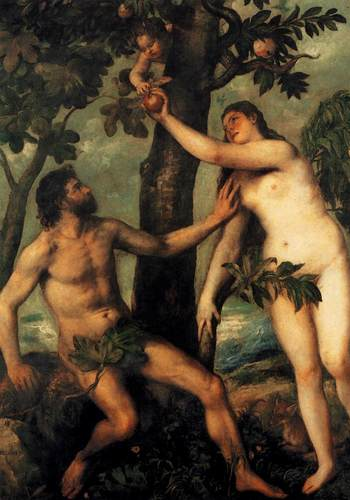
\includegraphics[width=.3\textwidth]{AdamEve.png}
\end{wrapfigure}

The practice of the destruction of this imagery leads to the next plane of awareness, the world of Formation. This is the task of concentration. However, this task is no longer experienced as toil; on the contrary it is effortless.

When Calm and Silence are achieved, we can enter into the world of Creation. Without Silence, knowledge require suffering: intellectual doubt, moral quandaries, illusions. However, in this state, gnosis is possible since a calm consciousness is the perfect reflection of the revelation from above.

In the fallen state, the World is experienced as oppressive, a system of unchanging laws, the plaything of ineluctable destiny. In the world of Creation, life returns, and the world is understood once again as a creative work of art. This means, in the end, that the Universe is Open. It cannot be encapsulated in any system of laws, or scientific theory, or in a philosophical system. This is how the project begins, although it never ends:

\begin{quotex}
The Arcana of the Tarot are magic, mental, psychic, and moral operations awakening new notions, ideas, sentiments, and aspirations, which means to say that they require an activity more profound than that of study and intellectual explanation. It is therefore in a state of deep contemplation --- and always ever deeper --- that they should be approached. And it is the deep and intimate layers of the soul which become active and bear fruit when one meditates on the Arcana of the Tarot. Therefore this ``night'', of which St. John of the Cross speaks, is necessary, where one withdraws oneself ``in secret'' and into which one has to immerse oneself each time that one meditates on the Arcana of the Tarot. It is a work to be accomplished in solitude and is all the more suitable for recluses.
\end{quotex}



\flrightit{Posted on 2022-11-03 by Cologero}

\begin{center}* * *\end{center}

\begin{footnotesize}
\begin{sffamily}
\texttt{Santiago on 2023-10-30 at 13:31 said:}

``Instead of toil, there was mystical spontaneity.''

I `let go' and thoughts appear all by themselves: first discursively, then as images and sounds. If angels are personified ideas, they can be quite pleasant to `speak with'. If I am more attuned to negativity, they may be demons, and so the effortlessness of concentration takes a backstep, as the spiritual combat must start here.

``Learning through suffering replaced direct revelation and gnosis.''

Through the ability of letting go, a new life plays out `before my eyes'. The thoughts--images--take on a reality all their own.

``Death entered the domain of life and sacred, creative magic.''

What is death to the outside world, is its own realm of unhindered, unitive and absolute freedom. Nevertheless, I must return to multiplicity, which is also its own kind of death.

\hfill

\texttt{Santiago on 2023-10-30 at 13:50 said:}

Apologies for double posting:

I struggle with the notion that every sensual thought or image is necessarily `bad'. Rather, I think it's just a matter of perspective:

``In the fallen state, the mind is perturbed with the spontaneously arising fluctuations of sensual and intellectual imagery. In this state, the mind is attached to the lowest plane of toil, suffering, and death, as it cannot conceive of anything superior.''

From that `superior viewpoint', they must clearly have value. The fireman who considers how to rescue the cat from the tree is not oppressed with `demonic' thoughts.

\hfill

\texttt{Taivasvaeltaja on 2023-11-06 at 10:42 said:}

This came out from the archives the right time since I'm composing an essay on the Fall and its meaning.


\hfill

\end{sffamily}
\end{footnotesize}

